\section{Laboratory setup}
\label{sec:setup}

Our setup consists of three primary components: the \SD telescope, a large area photodiode employed as a calibration reference, and the CBP
which illuminates either one or the other. In the following section, we will describe each component and detail their operations.

In comparison to the original CBP design outlined in \cite{Mondrik_2023}, a significant enhancement is the use of a solar cell to calibrate and monitor the CBP optical transmission between the optical sphere and the telescope output. Other noteworthy improvements include (1) replacing the laser light source from NIST with an EKSPLA NT 252, which offers a slightly more favorable wavelength power cutoff, (2) implementing a filtering system to prevent laser harmonics from being injected into the light beam and (3) synchronizing the photocurrent readings with laser light emission, facilitating the extraction of the signal, (4) replacing the Hasselblad camera by a Ritchey-Chretien telescope as collimating optics in order to remove all chromatic effects and enlarge the illumination region.	

\subsection{\SD}
\label{sec:stardice}

The \SD photometric instrument consists of a Newton telescope with a primary mirror of \SI{40}{\centi\meter} diameter (16'') and \SI{1.6}{\meter} focal length ($f/D = 4$). The focal plane hosts an Andor Ikon-M DU934P-BEX2-DD camera, equipped with a deep depleted and back-illuminated CCD sensor (E2V DU934P). The active area of the sensors is $\SI{13.3}{\milli\meter}\times\SI{13.3}{\milli\meter}$ divided in $1024\times 1024$ square pixel of \SI{13}{\micro\meter} side. In this baseline setup, the pixel resolution is \SI{1.68}{\arcsec} and the field of view $\SI{28.6}{\arcmin}\times\SI{28.6}{\arcmin}$.

A 9-slots \SI{28.5}{\milli\meter} filter wheel in front of the camera features 6 interference filters in the $ugrizy$ photometric system, a Star Analyser 200 diffraction grating, and a \SI{0.2}{\milli\meter} pinhole. The remaining slot is left empty. Aside the optional filters, the only other glass part in the light-path is the non-coated fused-silica window of the CCD cell\footnote{The manufacturer code for
  this window is WN35FS(BB-VV-NR)W}. The two sides of the window are affected by a \SI{0.5}{\degree} wedge.

The z-position of camera-filter wheel assembly is adjustable over \SI{9}{\centi\meter} allowing to focus from distances as close as \SI{35}{m} up to infinity. The 11cm diagonal flat is oversized to ensure the fully-illuminated plane extends over the sensor with a comfortable margin in all optical configurations. A model of the baffling and optics of the instrument build upon the batoid\footnote{\url{https://github.com/jmeyers314/batoid}} raytracing software has been tuned on pinhole images and is described in a companion technical note \cite{}.

In operation, the camera sensor is thermoelectrically cooled-down to a temperature of \SI{-70}{\celsius}, delivering a median dark-current of
\SI{0.15}{e^-/s}, neglected for the $\sim 1s$ exposures considered in this study. When operated in the lab, the telescope was mounted on a custom altazimuth mount to enable easy alignment with the CBP.

\subsection{Collimated Beam Projector}
\label{sec:cbp}

The Collimated Beam Projector (CBP) general setup needs the following: a tunable monochromatic light source, and an optic device able to recreate a parallel beam from a point source. In our case, the light source is an Ekspla NT252 tunable laser, using a Q-switched pump laser at \SI{532}{\nano\meter} and non-linear crystals to produce powerful monochromatic pulses from 335 to \SI{2600}{\nano\meter}. The pulse duration is fixed and lies between 1 and \SI{4}{\nano\second} with an energy of \SI{1.1}{\milli\joule} in the near infrared. The energy can be decreased at will by a factor of 2 using the tuning of the Q-switch (namely QSW in the following) which degrades the quality factor of the resonant cavity. Pulses are shot with a fixed frequency of \SI{1}{\kilo\hertz} and can be shot in two modes. The first one is called the "continuous mode", since it shoots pulses continuously with a \SI{1}{\kilo\hertz} frequency, while the second one is said "burst mode", sending packets of pulses by bursts. Each burst is composed from 1 to 1000 pulses, meaning the duration of a burst is restrained between \SI{1}{\milli\second} to \SI{1}{\second}. The pulses have a maximum linewidth below \SI{10}{\per\cm}, which can be converted into a maximum spectroscopic width below \SI{0.4}{\nano\meter} around \SI{600}{\nano\meter}. This is an upper limit quoted by the manufacturer, but measurements taken using a similar laser show bandwidths going from \SI{0.08}{\nm} to \SI{0.48}{\nm} in the 350 to \SI{1100}{\nm} range \citep{woodward2018}. The standard deviation of pulse energy is around 2.5\%. This laser is composed of three different operational configurations, from 335 to \SI{669}{\nano\meter}, from 670 to \SI{1064}{\nano\meter} and above \SI{1064}{\nano\meter}, which results in three different regimes of power and light contamination in the CBP. This laser was chosen for the offered wide wavelength range and the high pulse energy, as the source power is an important criteria for the CBP calibration with the solar cell, our reference calibration photodiode (see Section~\ref{sec:solarcell}). 

The laser output is polluted by light coming from the pump laser of other resonances in the system, both spatially and chromatically. The spatial pollution is stopped with a diaphragm. On the other hand, a filterwheel which contains three different broad bandpass filters is purifying the laser light from pump photons or other parasite signal. In particular, we use a red-pass filter RazorEdge LP03-532RU-25 to filter out the \SI{532}{\nano\meter} pump photons in the regime 645 to \SI{1074}{\nano\meter}, and a infrared-pass filter RazorEdge LP02-1064RU-25 above \SI{1074}{\nano\meter} to filter $<\SI{1064}{\nano\meter}$ photons appearing in this regime. We also use a blue-pass filter BrightLine Multiphoton FF01-680/SP-25 in the regime 530 to \SI{645}{\nano\meter} to remove a contamination not detected in the spectrograph and which we were not able to identify. A black metallic box encloses the entire optical stage to minimize light scattering in the room.

Being filtered, the light is focused and injected into an optical fiber Thorlabs MHP910L02 with a wide core diameter of \SI{910}{\micro\meter}, which is plugged into an IS200-4 $\Phi$2'' integrating sphere from Thorlabs, which has an internal \SI{50}{\mm} diameter and is composed of 1 input and 4 output ports. The integrating sphere dilutes the flux, breaks the laser light coherence, and eliminates  any spatial dependance to achieve a uniform surface brightness. Two monitoring instruments are plugged on the sphere. First a silicon photodiode Thorlabs SM05PD3A with a high efficiency in the UV is mounted on an output port orthogonal to the laser input port to control the laser power stability. It is mounted behind a pinhole to reduce the photon flux and ensure that it works in its linear regime. It is read by a Keithley 6514 electrometer at a rate of \SI{50}{\hertz}. Additionnaly, an OceanOptics Q65000 fiber spectrograph is plugged on another output to monitor the true laser wavelength and the spectral purity. One port is left free to plug a calibration lamp to calibrate the spectrograph when needed. Finally, a slider with pinholes of different diameters is mounted on the output port connected to the CBP optics. Figure~\ref{fig:sphere} shows a schematic of the integrating sphere and the instruments plugged into it.

We used three different pinholes, of diameter \SI{75}{\micro\meter}, \SI{2}{\milli\meter} (respectively P75HK and P2000HK from Thorlabs) and \SI{5}{\milli\meter} (homemade). The \SI{5}{\mm} pinhole is the largest possible given the \SD field of view, and gives the maximum flux. The other pinholes are used for systematic checks and filter edge analysis. The pinhole slider is attached to the ocular of a 154/1370 Ritchey-Chrétien Omegon telescope in order to position the pinhole at the focal point of the optics. The light injected in the telescope mounted backward will project a parallel and collimated beam. An iris diaphragm is positioned \SI{16}{mm} after the pinhole and adjusted to cut light that would otherwise miss the secondary mirror of the telescope. A small amount of light scatters on the iris blades and is best observed in telescope images of the CBP taken with the \SI{2}{mm} pinhole configuration. In these images, it forms a faint ring with a radius of approximately \SI{340}{pixels}, discinct from the main spot. When comparing annular photometry of the ring to that of the main spot, the fraction of scattered light is usually smaller than \num{6e-4} between 400 and \SI{900}{nm}.

The whole assembly is mounted on a robotic Celestron NexStar Evolution 6 altazimuth mount. As a last step, we cropped the output of the Ritchey-Chrétien Omegon with a mask shaped as a quarter of a disk corresponding to one quadrant of its secondary mirror spider, so that the actual beam shape is only a fourth of the complete aperture. This ensure that the entire beam can fit inside the reference solar cell footprint.

\begin{figure}
    \centering
    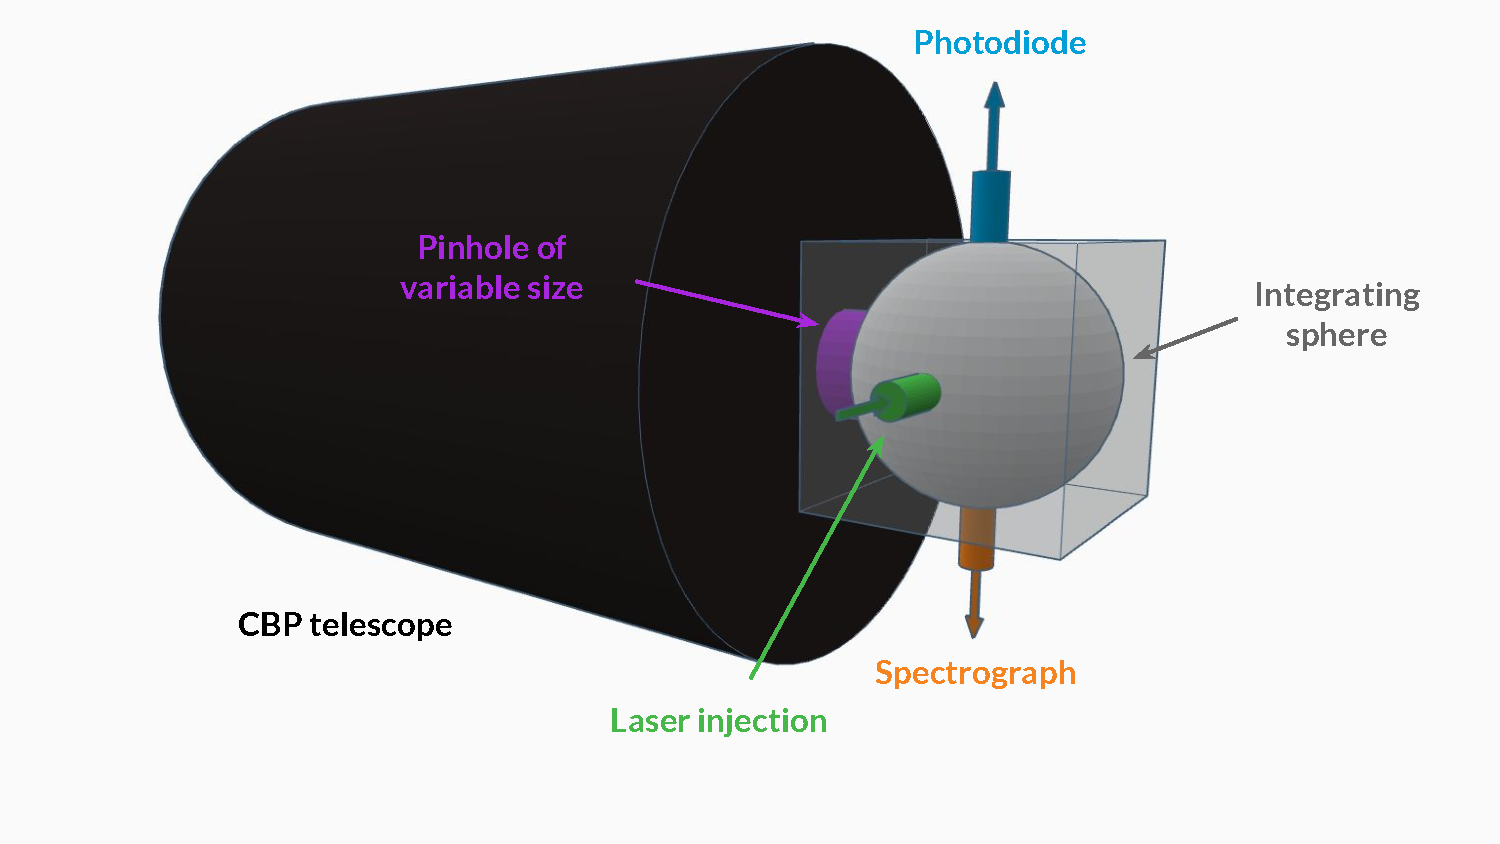
\includegraphics[width=1\columnwidth]{fig/integrating_sphere_3d.pdf}
    \caption{Schematic of the integrating sphere}
    \label{fig:sphere}
    %Tinkercad
\end{figure}

\begin{figure*}[ht]
\centering
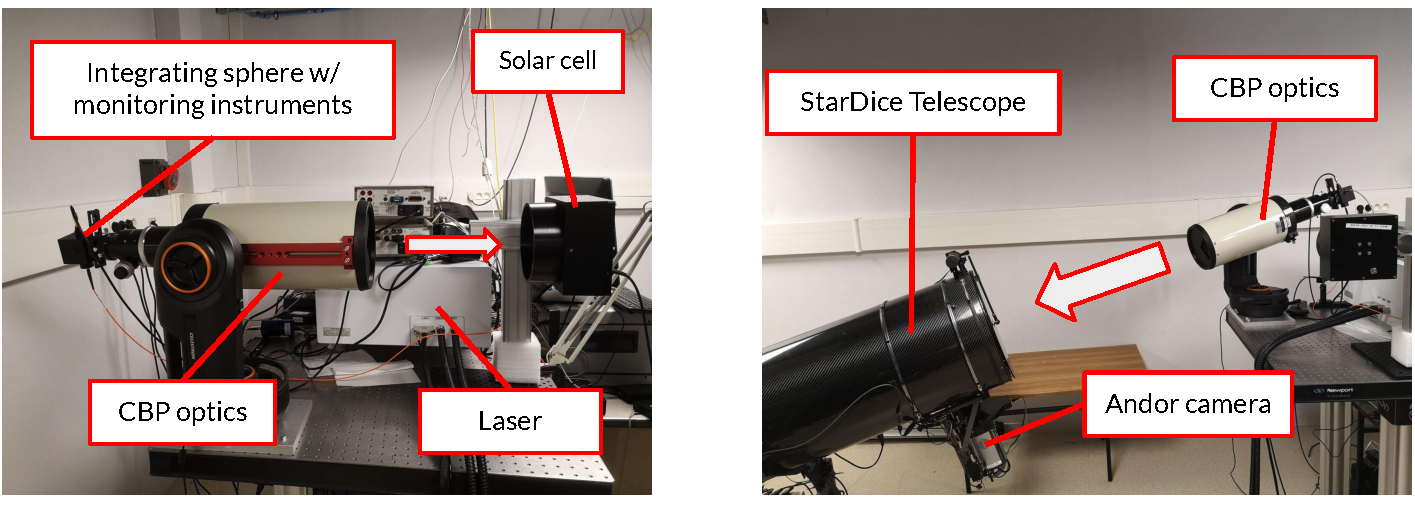
\includegraphics[width=\textwidth]{fig/cbp_setup_cropped.pdf}
\caption{Pictures of the different CBP setups. Left: CBP setup when shooting in the solar cell. Right: CBP setup when shooting in the \SD telescope.}
\label{fig:cbp_setup}
\end{figure*}

\subsection{Solar cell description}
\label{sec:solarcell}

We use a C60 solar cell of 3$^{\mathrm{rd}}$ generation from Sunpower as our calibration reference. Its sensitive area forms a square with \SI{12.5}{\centi\meter} side, setting the maximum size of the CBP beam which can be accurately calibrated. This solar cell is set on a two-axis mount, one that allows a movement in the direction of the optical axis of the CBP telescope, and another axis that is vertical, which allows to adjust the height of the solar cell. It is placed at \SI{16}{\cm} approximately from the telescope aperture. This solar cell is connected via a coaxial cable to a Keysight B2987A electrometer, the same that was used for its calibration. The charges are measured at a rate of \SI{500}{\hertz}. In Figure~\ref{fig:cbp_setup} right, we show a picture of the setup when the CBP is aiming at the \SD telescope described in section~\ref{sec:stardice}.


\subsubsection{Quantum efficiency measurement}
 
The quantum efficiency (QE) as a function of wavelength for the solar cell was measured relative to a NIST-calibrated photodiode by using a monochromator as a light source and using an electrometer to measure the current of the solar cell and of the photodiode at each wavelength. The monochromator wavelength was calibrated with a spectrograph relative to a mercury calibration source. Details of the setup are discussed in ~\cite{solarcell}. The quantum efficiency of the solar cell used for these measurements is shown in Fig.~\ref{fig:sc_qe}. Five measurements were taken per source wavelength with a \SI{1}{\nm} step. The smoothed average per wavelength is reported in Fig.~\ref{fig:sc_qe}. The uncertainty cited is from the RMS of the current measurements. The unexpected glitch at \textasciitilde\SI{550}{\nm} is masked by a linear interpolation. 

\begin{figure}[!h]
\centering
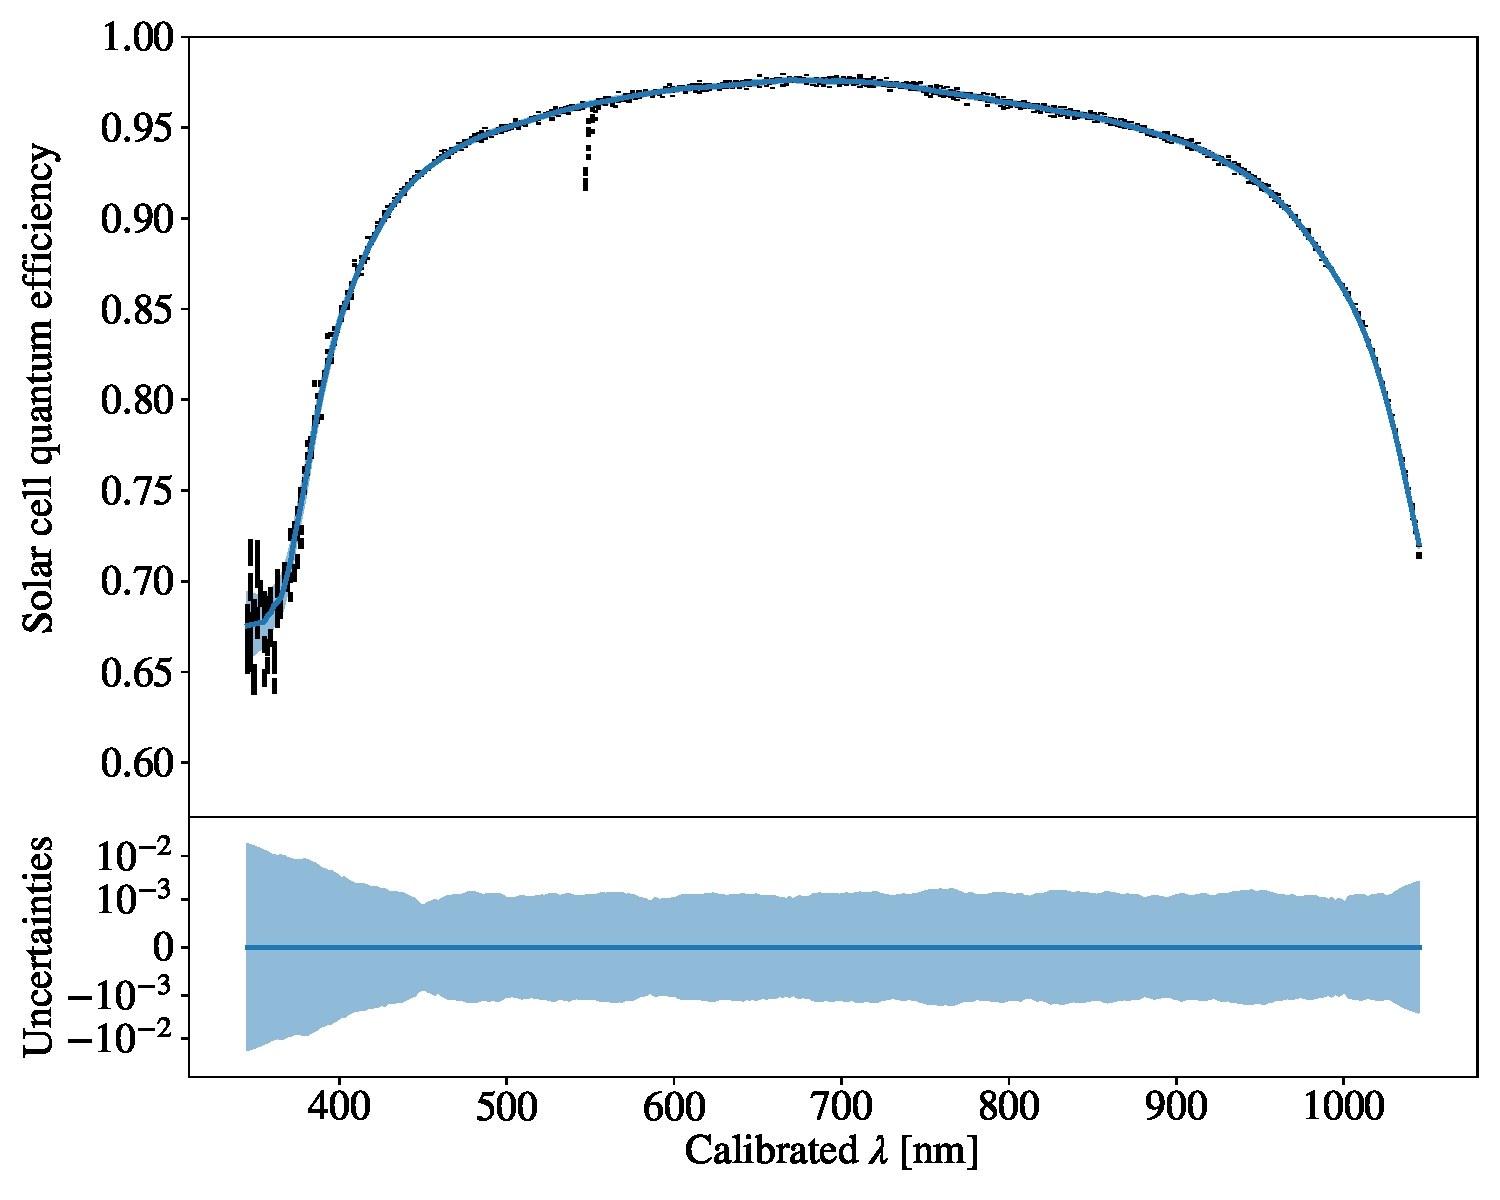
\includegraphics[width=\columnwidth]{solarcell_qe}
\caption{Solar cell quantum efficiency with respect to wavelength (top) and error bar sizes (bottom).}
\label{fig:sc_qe}
\end{figure}

The QE of the solar cell was measured within a temperature range from \SI{32}{\degreeCelsius} to \SI{39}{\degreeCelsius}. At longer wavelengths, the QE increased slightly as the temperature increased (see Fig.~\ref{fig:SC_temp}). This trend is consistent with the temperature dependence of silicon's QE \citep{Green_2008}. At 1050 nm, the QE changes by more than 0.1 percent per degree.
\begin{figure}[!h]
\centering
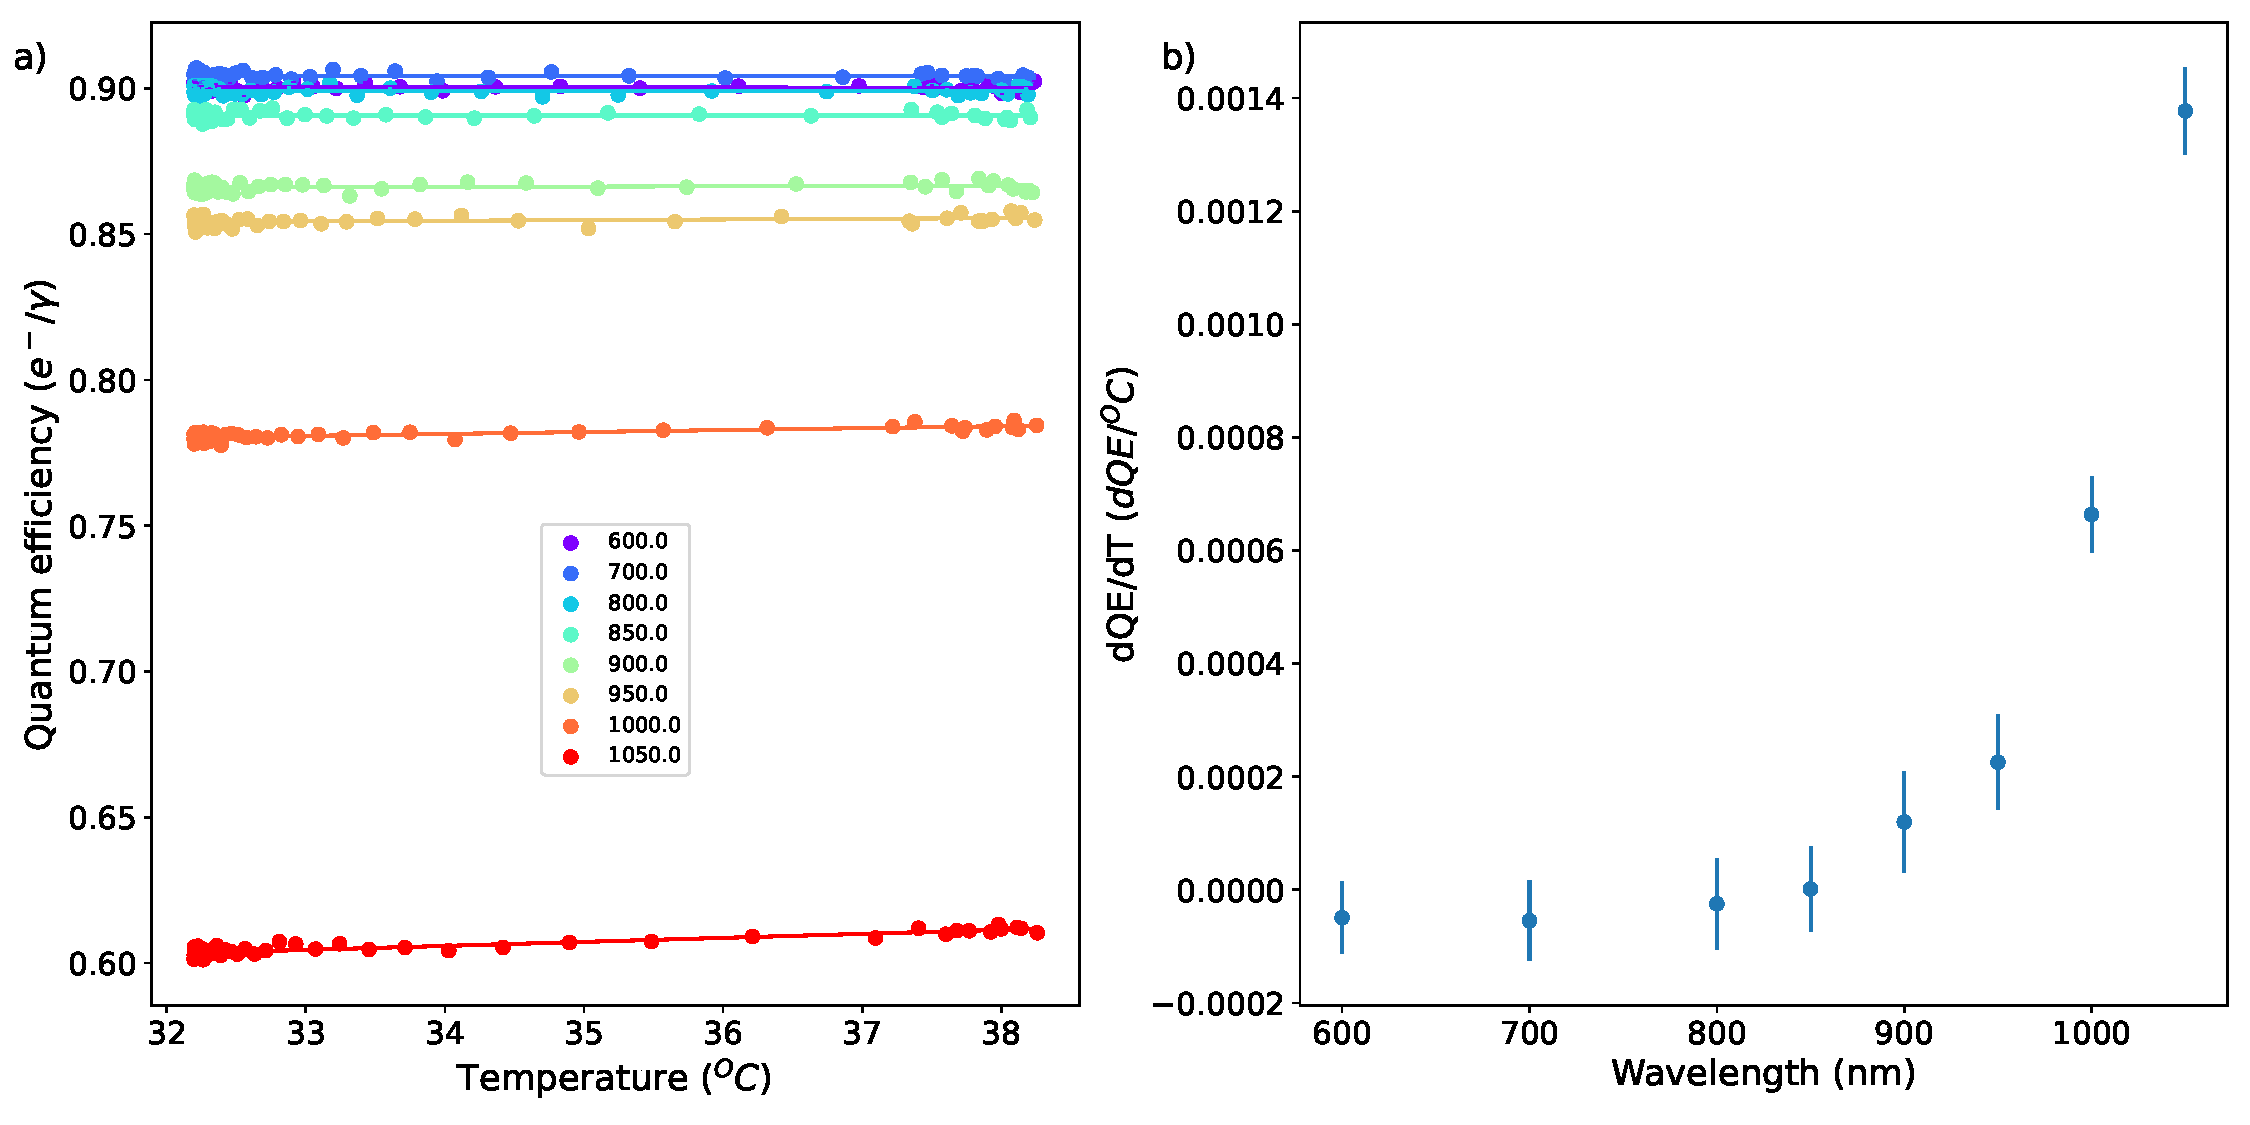
\includegraphics[width=\columnwidth]{SC_temp_dep.pdf}
\caption{(a) Solar cell quantum efficiency vs temperature for wavelengths ranging from 600 to 1050 nm. (b) Fitted change in quantum efficiency per degree Celsius for wavelengths ranging from 600 to 1050 nm.}
\label{fig:SC_temp}
\end{figure}

Additionally, the effect of the angle of incidence on the solar cell QE was measured. The solar cell was rotated up to 35 degrees off-axis. The results are shown in Fig.~\ref{fig:SC_angle}. There is a stronger dependence on angle of incidence at wavelengths that are less than 600 nm, but the change in QE for wavelengths greater than 400 nm is less than 5e-4 per degree.
\begin{figure}[!h]
\centering
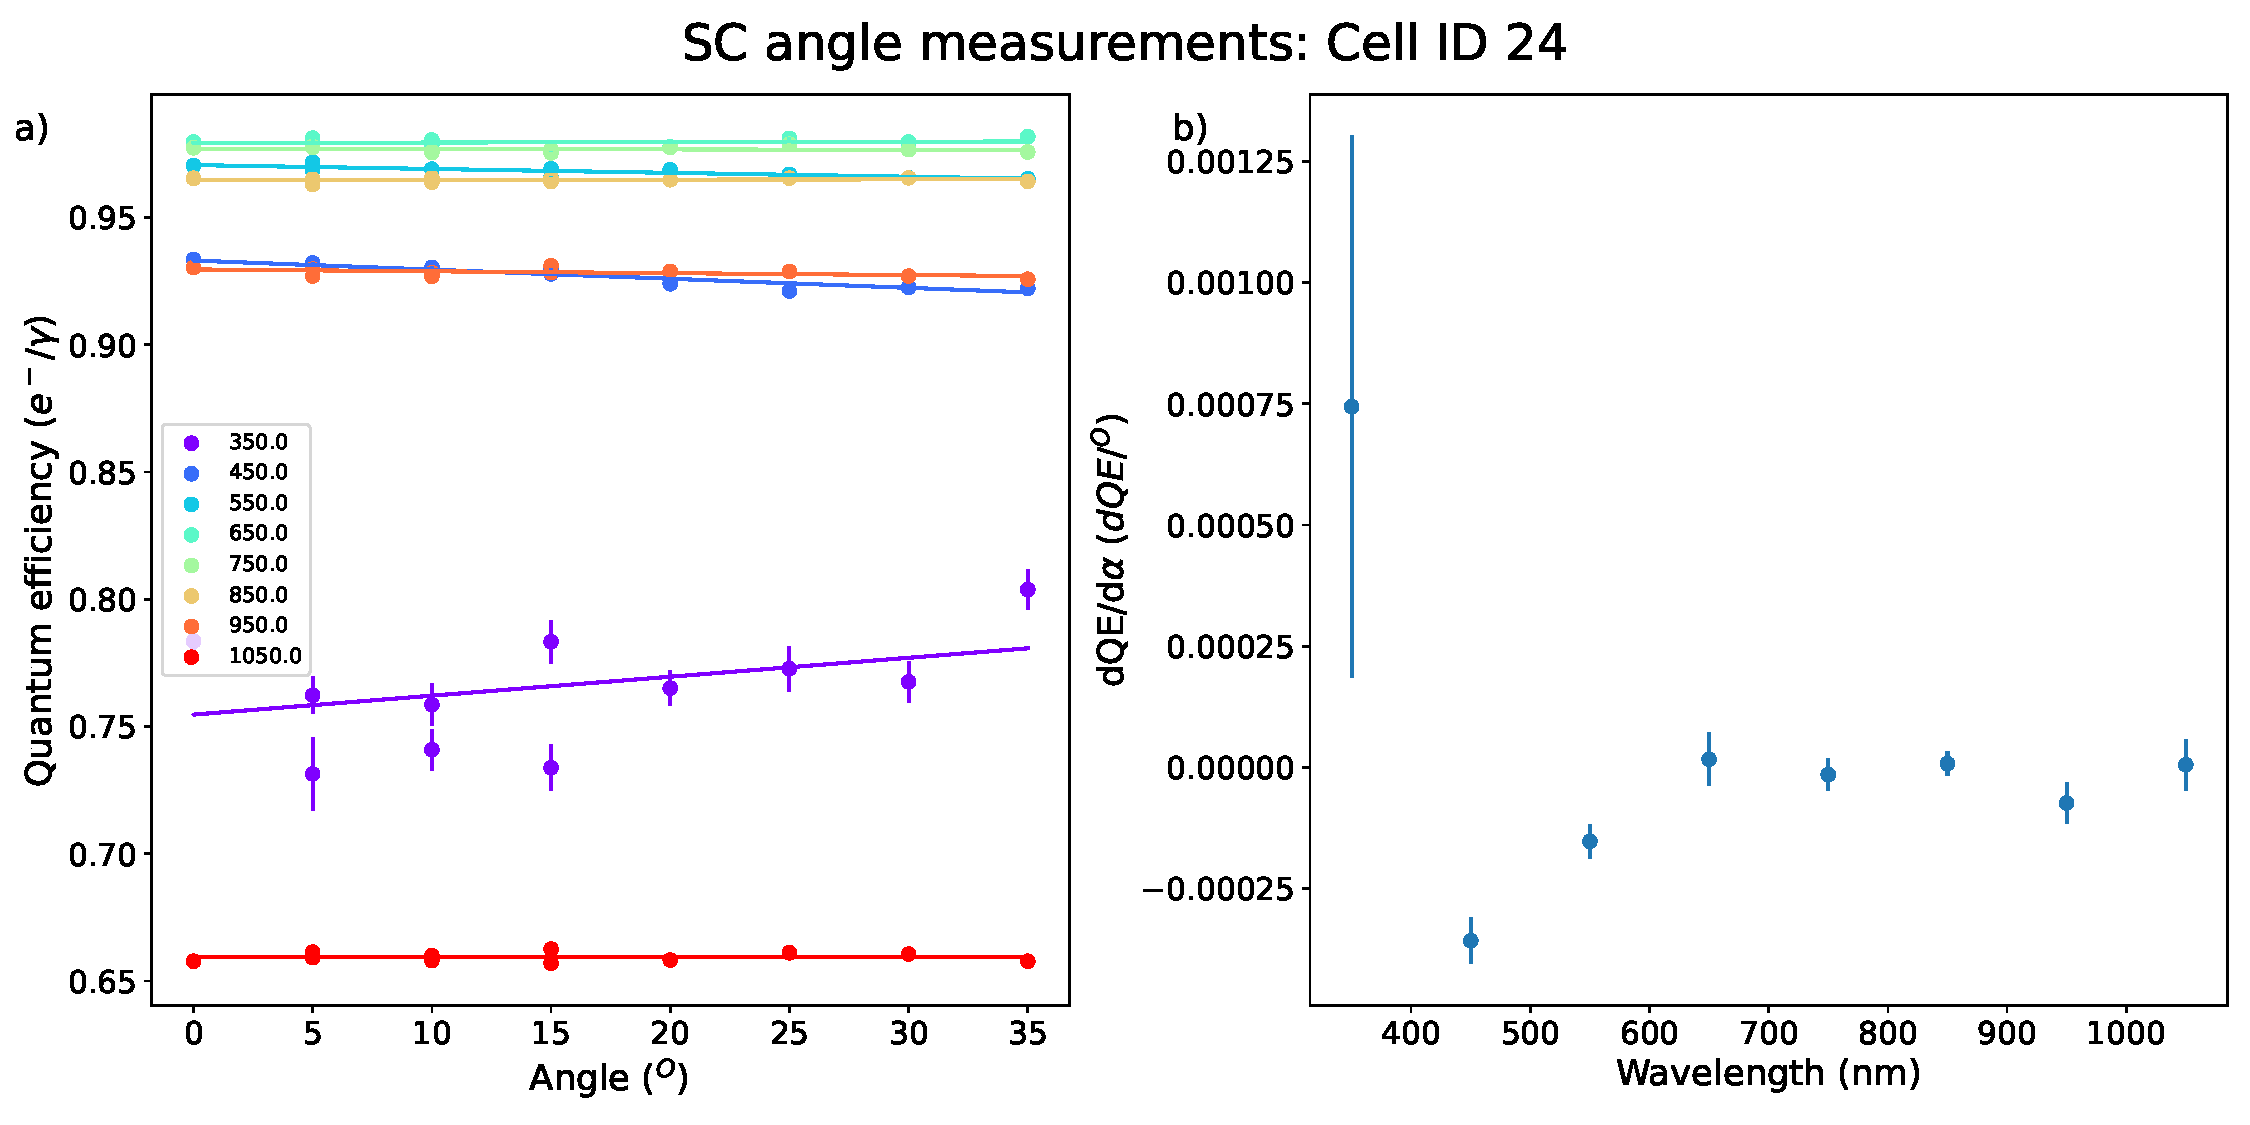
\includegraphics[width=\columnwidth]{SC_angle_dep.pdf}
\caption{(a) Solar cell quantum efficiency vs solar cell tilt relative to normal incidence for different wavelengths. (b) Fitted change in quantum efficiency per degree of solar cell tilt relative to normal incidence vs wavelength.}
\label{fig:SC_angle}
\end{figure}

The solar cell was aligned perpendicalular to the CBP output beam with a precision better than \SI{1}{\degree} and not moved during all the measurement campaign. Meanwhile, room temperature was monitored and has not varied more than \SI{2}{\degreeCelsius}.
%Considering measured variations of quantum efficiency with angle and temperature, we assumed that this systematic is well below the per-mill level and is not considered in the following of the paper. 

%\subsubsection{Current or charge mode}
%
%The charges in the photodiode and the solar cell are read with electrometers in charge mode. This mode is better than the current mode as the integration is performed in a capacitance. This avoids modeling the precise current timelines before integrating them numerically, as they are subtlety different from squarewave functions due to different time responses in the system and contaminated by random dark current fluctuations. 

%\begin{itemize}
%\item Ekspla NT252 tunable laser
%\item Light injection system with filters
%\item Optical sphere ref
%\item Ocean QE65000 spectrograph
%\item Photodiode + Keithley 6514. Fig \ref{fig:thorlabs_response}\\
%  \emph{Old one} (used in summer 2021 up to 14th of October 2021): Thorlabs
%  SM05PD1B with FDS100 spectral response data\\
%  \emph{New one} (replaced on the 14th of October 2021): Thorlabs SM05PD3A with
%  FD11A spectral response data

%\item Pinhole slider
%\item Telescope: Ritchey Chretien Omegon telescope\\
%  Apperture ratio $f/9$\\
%  Apperture $154 mm$ \\  
%\item Telescope mount
%\item Solar Cell on movable mount
%\item Keysight B2987A: in order to be able to chop the light at a higher frequency
%  than what the Keithley can do. And it is a more contemporary instrument.
%\end{itemize}
  
%\begin{figure}[!ht]
%    \begin{center}
%      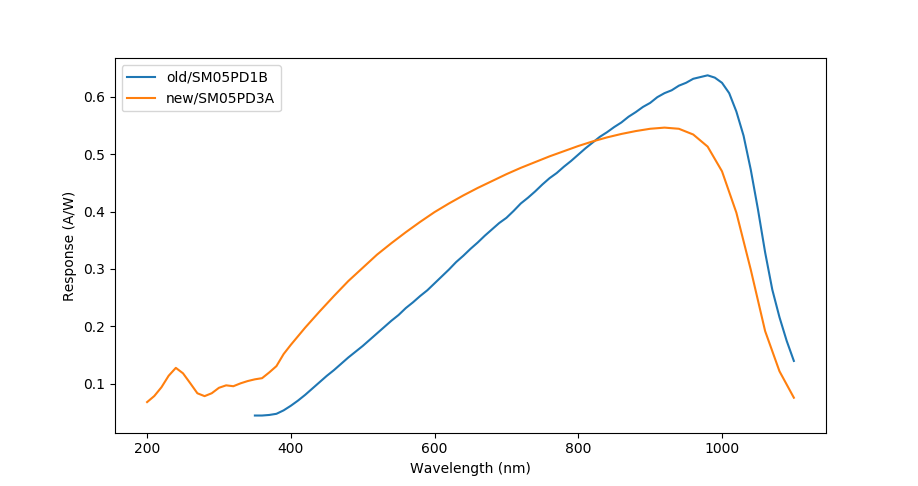
\includegraphics[width=0.8\columnwidth]{thorlabs_response}
%    \end{center}
%    \caption[]{Response curves of the photodiodes. We see the noticeable
%      improvement in the blue for the new one.}
%    \label{fig:thorlabs_response}
%\end{figure}

\subsubsection{Dark current characterisation}

Due to the low resistance of the solar cell, we observed a quite strong current even in dark conditions (about \SI{20}{\nano\ampere}). Therefore, we built a device that uses a precision voltage source with a tunable voltage divider to inject a counter-current that cancels this contribution. The current value was tuned to observe approximately no drift when using the Keysight in charge mode inside the usual acquisition time window ($< \SI{1}{\minute}$). Doing so, we avoided saturating the electrometer when using the solar cell in dark and laser-on conditions. 

%\begin{itemize}
%\item Without offset box: $\sim 20 nA$
%\item With offset box: $~ <0> nA \pm 5 nA$
%\end{itemize}
After cancelling the dark current drift, the analysis of the solar cell dark signal revealed a $1/f$ noise, with power line harmonics contributions at \SI{50}{\hertz},  \SI{100}{\hertz}, and \SI{150}{\hertz} (see Figure~\ref{fig:darkcurrentspectrum}). To investigate the source of the $1/f$ component in the power spectrum, we compared the output of the Keysight when connected to a resistor with the same value as the shunt resistance of the solar cell. We found that the two power spectra were identical, leading us to conclude that the fluctuations in the transimpedance amplifier bias voltage are the source of this $1/f$ noise. These fluctuations cause parasitic current to flow through the load resistance. By increasing the load resistance, we can decrease the amplitude of the resulting noise. Among a set of calibrated solar cells, we therefore chose the one with the highest shunt resistance ($R_{\rm shunt} = \SI{1.8}{\kilo\ohm}$), and limited the burst durations to at most 200 pulses (\SI{200}{\ms}). Doing so, in the burst time window, the Keysight noise is dominated by the power line harmonics whereas the random $1/f$ noise remains subdominant.

%cbp_paper_plots.py
\begin{figure}[h]
\begin{center}
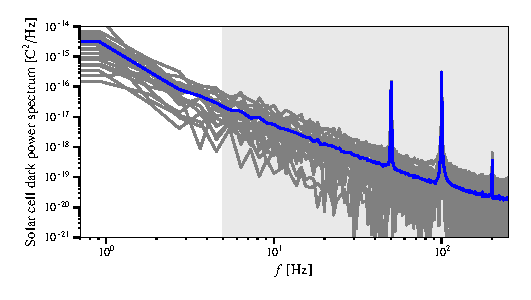
\includegraphics[width=1\columnwidth]{sc_dark_ps}
\end{center}
\caption[]{Solar cell dark current power spectrum for 20 runs without light in the solar cell (gray curves) and their average (blue). The light gray region encompasses expected noise spectrum contribution for \SI{200}{\ms} laser bursts.}
\label{fig:darkcurrentspectrum}
\end{figure}

\FloatBarrier   

\subsection{Time synchronisation}
\label{sec:synchro}

The precision of the analysis can be significantly improved if the laser pulses can be accurately identified within the photocurrent timeseries. This is particularly crucial for solar cell measurements, where signal-to-noise ratios are typically lower.

To accomplish such synchronization, we recorded the timing of all three trigger lines of the laser and both electrometers on a single microcontroller. Upon detecting a TTL pulse on any of these lines, the microcontroller registers a 32-bit timestamp using its internal clock counter, enabling synchronization with a resolution of 500 nanoseconds over extended durations (up to 2100 seconds). This custom synchronization device Arduino based, whose code is openly accessible \cite{logic_timer}, is referred to as the digital analyzer throughout the remainder of this text.

\subsection{Measurement principle}

Table~\ref{tab:quantities} sum up the three quantities that are measured with the two setups in Figure~\ref{fig:cbp_setup}.

\begin{table}
  \centering % used for centering table
  \caption{Definition of measured quantities in our \SD+CBP setup.}
    \begin{tabular}{M{1cm} M{7cm}} % centered columns (4 columns)
        \hline\hline % inserts double horizontal lines
        Name & Description \\
        \hline
        \bf{$\Qphot(\lambda)$} & The charge per burst collected by the integrating sphere monitoring photodiode, measured by the Keithley 6514 in Coulomb \\

        \bf{$\Qsolar(\lambda)$} & The charge per burst collected by the solar cell, measured by the Keysight 2987A in Coulomb \\
        \bf{$\Qccd(\lambda)$} & The charge collected by the Andor CCD camera of the \SD telescope in ADU. \\
        \hline %inserts single line
    \end{tabular}
    \label{tab:quantities} % is used to refer this table in the text
\end{table}

First, we need to measure the response of the CBP optics $\Rcbp(\lambda)$ by shooting into the calibrated solar cell as shown in Figure~\ref{fig:cbp_setup} left. It is computed with the Equation~\ref{eq:rcbp}. In this equation, we know the quantum efficiency of the solar cell $\Esolar$ from Figure~\ref{fig:sc_qe}, and $e$ is the elemental charge of the electron.

\begin{equation}
    \Rcbp(\lambda) = \frac{\Qsolar(\lambda)}{\Qphot(\lambda) \times \Esolar \times e}.
    \label{eq:rcbp}
\end{equation} 

Once we have this response, we can shoot inside the \SD telescope as show in Figure~\ref{fig:cbp_setup} right, and obtain $\Rtel(\lambda)$ with the Equation~\ref{eq:rsd}.

\begin{equation}
    \Rtel(\lambda) = \frac{\Qccd(\lambda)}{\Qphot(\lambda) \times \Rcbp(\lambda)}.
    \label{eq:rsd}
\end{equation}

We will focus on $\Rcbp(\lambda)$ and $\Rtel(\lambda)$ respectively in sections \ref{sec:rcbp} and \ref{sec:rsd}.

\subsection{Measurement overview}
\label{sec:strategy}

The schedule for all measurements conducted to determine $\Rtel(\lambda)$ and estimate associated systematic uncertainties is outlined in Table~\ref{tab:schedule}. Each row in the table corresponds to a specific hardware configuration and measurement run. We have assigned labels to each run and specified the following details: (1) the target of the CBP, (2) the pinhole used in the CBP slide, (3) the QSW setting for the laser, (4) the filters used in the \SD camera filter wheel (when applicable), (5) any specificities of the measurement, and (6) the number of runs.

The campaign of measurement has started and ended with a calibration of the spectrograph. A calibration Hg-Ar lamp was plugged into the integrating sphere and its light was measured with the spectrograph. This corresponds to lines No.~1 and No.~13 of the Table~\ref{tab:schedule}.

Two different pinholes in the CBP slides were used for these measurements. When shooting into the \SD telescope, the \spinhole pinhole forms a point-like image of about 10 pixels in diameter well suited for photometry while avoiding issues related to ghosting. When shooting into the solar cell, the \bpinhole pinhole is necessary to achieve good signal-to-noise ratio. Since $\Rcbp(\lambda)$ depends slightly on the pinhole diameter, we also need to intercalibrate the two responses $R_\mathrm{CBP}^{\mathrm{\SI{5}{\milli\meter}}} (\lambda)$ and $R_\mathrm{CBP}^{\mathrm{\SI{75}{\micro\meter}}} (\lambda)$. This intercalibration can be performed thanks to the measurements in line No.~8 of Table~\ref{tab:schedule}.

A major issue with the CBP is that its output light does not illuminate the entirety of the \SD primary mirror as an astrophysical source would do, but only a portion of it. It is necessary to perform a \textit{pupil stitching} to reconstruct the transmission of the mirror, by combining the measurement of $\Rtel(\lambda)$ when shooting at different positions on the mirror. When doing so, only the point of impact on the mirror is modified, but the point of incidence on the focal plane is the same. The different positions are shown in Figure~\ref{fig:8_mirror_positions}. The pupil stitching corresponds to lines No.~2 and No.~3 of Table~\ref{tab:schedule}. The method used to perform the pupil stitching is detailed in Section~\ref{sec:pupil_stitching}.

To check the uniformity of the \SD focal plane, a measurement of $\Rtel(\lambda)$ at 16 different positions on the focal plane has been performed. Only the position on the focal plane is modified while the point of impact on the mirror stays the same. This dataset corresponds to the line No.~12 of Table~\ref{tab:schedule}. 

Finally, some systematic measurements have been carried out. A cap has been placed on the CBP output to measure the background of the room for both setup configurations, corresponding to lines No.~9 and No.~10 of Table~\ref{tab:schedule}. A measurement of the scattered light is possible with the dataset No.~11, by shifting the position of the solar cell from the CBP output of approximately \SI{16}{\centi\meter}.


\begin{table*}[t]{}
  \centering
  \caption{Detailed schedule of the measurements.}
    \begin{tabular}{M{.25cm} M{3cm} M{1.6cm} M{1.1cm} M{1.4cm} M{3cm} M{4cm} M{1.25cm}}
        \hline\hline
         \bf{N$^{\circ}$} & \bf{Label} & \bf{Target} & \bf{Pinhole} & \bf{QSW} & \bf{\SD bands} & \bf{Specificity} & \bf{Number of runs} \\ 
         \hline
         1 & Wavelength calibration & Spectrograph & - & - & - & Hg-Ar lamp light source & 1 \\ 
         
         2 & Radial pupil stitching & \SD & \SI{75}{\micro\meter} & MAX & \shortstack{u, g, r, i, z, y, \\ EMPTY, GRATING} & 4 mirror radial positions & 1 per position \\
         
         3 & Quadrant pupil stitching & \SD & \SI{75}{\micro\meter} & MAX & EMPTY & 4 mirror  quadrant positions  & 1 per position \\
         
         4 & Repeatability measurement & \SD & \SI{75}{\micro\meter} & MAX & \shortstack{u, g, r, i, z, y, \\ EMPTY, GRATING} & Fixed mirror and focal plane position & 3 \\
         
         5 & CBP response calibration before & Solar cell & \SI{5}{\milli\meter} & 298, MAX & - & CBP monitoring before \SD measurements & 5 \\
         
         6 & \SD main calibration & \SD & \SI{5}{\milli\meter} & MAX & \shortstack{u, g, r, i, z, y, \\ EMPTY, GRATING} & Fixed mirror and focal plane position & 5 \\
                  
         7 & CBP response calibration after & Solar cell & \SI{5}{\milli\meter} & 298, MAX & - & CBP monitoring after \SD measurements & 5 \\
         
         8 & Pinholes inter-calibration & \SD & \SI{75}{\micro\meter}, \SI{2}{\milli\meter}, \SI{5}{\milli\meter} & MAX & EMPTY & 3 different pinhole sizes & 1 per pinhole \\
            
         9 & \SD background measurements & \SD & \SI{5}{\milli\meter} & MAX & EMPTY & Cap on CBP output & 1 \\
            
         10 & Solar cell background measurements & Solar cell & \SI{5}{\milli\meter} & MAX & - & Cap on CBP output & 2 \\
            
         11 & Solar cell distance calibration & Solar cell & \SI{5}{\milli\meter} & 298, MAX & - & 2 solar cell positions at \SI{16}{\centi\meter} relative distance & 1 per position \\
            
         12 & Focal plane measurement & \SD & \SI{75}{\micro\meter} & MAX & EMPTY & 4x4 grid positions on the \SD focal plane & 1 per position \\
           
         13 & Wavelength calibration & Spectrograph & - & - & - & Hg-Ar lamp light source & 1 \\ 
         \hline
    \end{tabular}
    \label{tab:schedule}
\end{table*}


\begin{figure}[!h]
\centering
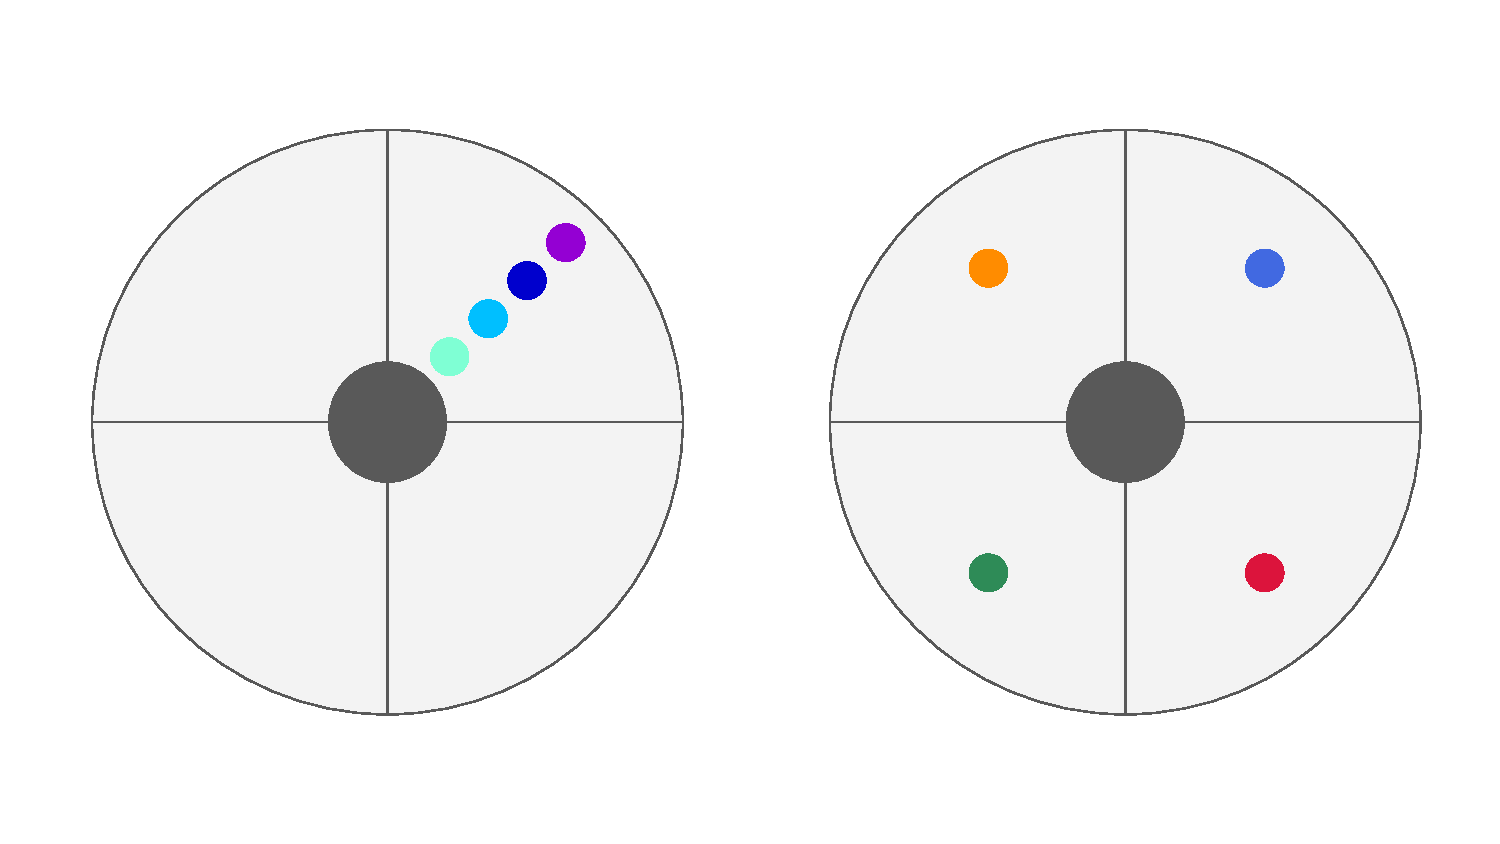
\includegraphics[width=\columnwidth]{fig/8_mirror_positions.pdf}
\caption{Left: Schematic of the 4 different radial relative positions on the primary mirror of the \SD telescope. Right: Schematic of the 4 different quadrant relative positions on the primary mirror of the \SD telescope.}
\label{fig:8_mirror_positions}
\end{figure}

\begin{figure}
	\centering
\end{figure}
\com{!!!TO BE REMOVED!!!}

%\begin{figure}
%    \centering
%    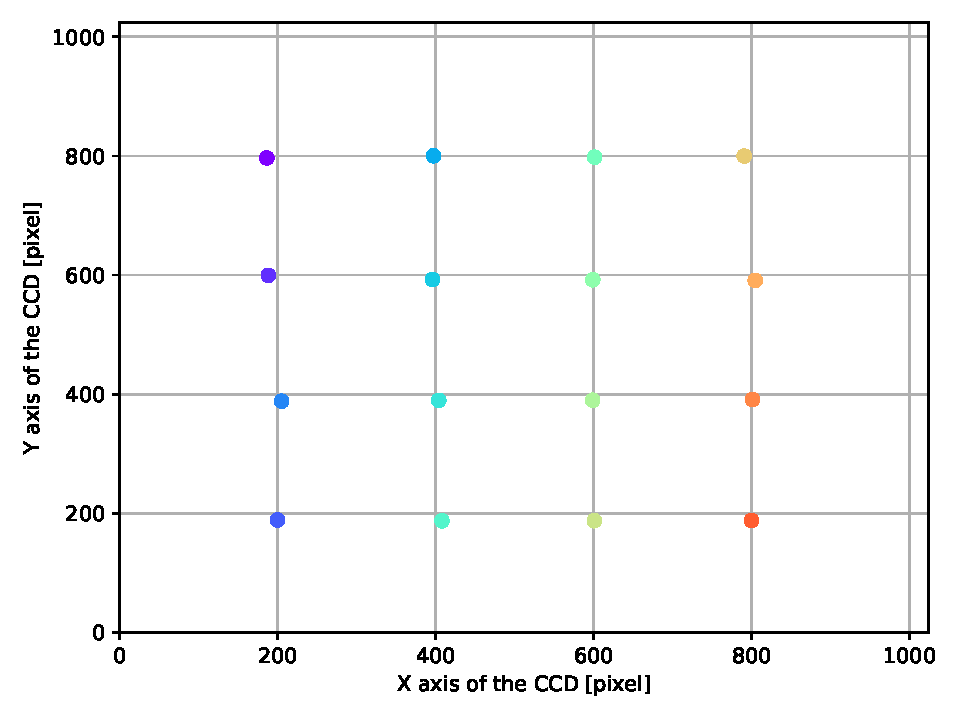
\includegraphics[width=\columnwidth]{fig/ccd_grid_colors.pdf}
%    \caption{Schematic of the (4x4) grid positions on the \SD CCD focal plane.}
%    \label{fig:ccd_grid}
%\end{figure}

%\newpage
